\documentclass[10pt]{article}

\usepackage{polski}
\usepackage{graphicx}
\usepackage{hyperref}
\graphicspath{{images/}}

\usepackage{geometry}
\newgeometry{tmargin=4cm, bmargin=4cm, lmargin=3.2cm, rmargin=3.2cm}

\usepackage{fancyhdr}
\pagestyle{fancy}



\begin{document}

\begin{titlepage}


\begin{center}

  \LARGE \textsc{Politechnika Wrocławska}\\
  \vspace*{0.2cm}
  \Large \textsc{Wydział Informatyki i Telekomunikacji}\\
  \vspace*{0.4cm}
  \centering
\includegraphics[width=0.2\textwidth]{WITlogo.png}\\
  \vspace*{0.2cm}
  \vspace*{2cm}

  \centerline{\rule{\textwidth}{1.2pt}}
  \vspace{0.4cm}
  \Huge\textbf{Metody i Systemy Decyzyjne}
  \centerline{\rule{\textwidth}{1.2pt}}
  \vspace{1cm}
  \LARGE Sprawozdanie z laboratorium\\
  \vspace{3.5cm}
  \textsc{Autor}\\
  \vspace{0.2cm}
  \textbf{Kacper Wójcicki}\\
  \vspace{0.1cm}
  \Large nr albumu: \textbf{260388}\\
  \vspace{0.1cm}
  kierunek: \textbf{Informatyka Stosowana}

  \vspace*{\fill}
  \Large \textit{\today}

 \end{center}


\end{titlepage}


\begin{abstract}
%Celem \textbf{pracy} \textit{jest}, \underline{zeby} prowadzący się cieszył. Dane do badań zostały pobrane z Ministerstwa Prawdy. Analizę przeprowadzono z wykorzystaniem modelu zstępującego. W rezultacie symulacji wielokrotnej udało się ustalić, że co trzeci Polak jest przekonany, że jest co drugim Polakiem.
Celem pracy jest zbadanie wpływu alkoholu na takie czynniki życiowe jak szczęście, długość życia i PKB per capita.
Dane zostały pobrane dla 144 krajów z wikipedi.
Analizę przeprowadzono za pomocą regresjii liniwej oraz regresji wielomianowej 4 stopnia dla dokładniejszych wyników
W rezultacie udało się stwierdzić, że istnieje pewna zależność między alkoholem, a wyżej wymienionymi czynnikami życiowymi
\end{abstract}

\section{Wstęp -- sformułowanie problemu}
\label{sec:wstep}

%Z zachorowaniami jest tak, że nigdy nie wiadomo kto kogo. W ramach pracy utworzona zostanie sieć kontaktów wzajemnych w oparciu o bazę danych udostępnionych na stronie Ministerstwie Prawdy. Podjęta zostanie próba wywnioskowania z otrzymanej sieci informacji kto z kim, kiedy i gdzie.
W naszych badaniach chcemy ukazać jak alkohol wpływa na nasze życie.
W tym celu pobraliśmy dane o średniej liczbie litrów alkoholu wypitych przez ludzi oraz dane takie jak:
\begin{enumerate}
    \item współczynnik szczęścia
    \item średnia długość życia
    \item PKB per capita
\end{enumerate}

\section{Opis rozwiązania}

%Dane kto kogo zostaną pobrane ze strony \url{www.minpra.gov.pl}. Dostęp do danych uzyskano metodą na rympał. Baza została zapisana w postaci ramki danych biblioteki \texttt{Pandas}. Zawiera ona informacje o 43440 osobach w wieku od 12 do 68 lat, licząc od urodzenia.

%Wyznaczono odwzorowanie relacji \textit{kto kogo} na \textit{kto z kim} za pomocą wzorów Cramera, z których następnie uzyskano zbiór wartości własnych, a z całości obliczono wyznacznik trzeciego stopnia, będący rozwiązaniem postawionego problemu. Analogicznie wyznaczono relacje \textit{kto kiedy} i \textit{gdzie z kim}, przy czym odpowiednio do rodzaju relacji dobrany został stopień wyznacznika, a wartość stałej Laplace'a estymowano w drodze symulacji Monte Carlo.

Dane o wyżej wymionych czynnikach zostały pobrane z ogólnodostępnego źródła jakim jest wikipedia, a dokładnie ze stron podanych poniżej
\begin{itemize}
    \item \url{www.wikipedia.pl}
    \item \url{www.wikipedia.pl}
    \item \url{www.wikipedia.pl}
    \item \url{www.wikipedia.pl}
\end{itemize}
Z tabel wzięte zostały potrzebne kolumny oraz umieszczone w ramkach danych biblioteki \texttt{Pandas}.
Dla każdego z czynników (współczynnik szczęścia, średnia długość życia oraz PKB per capita) zostały stworzone osobne zależności od alkoholu wypitego na osobę poprzez użycie regresji liniowej oraz regresji wielomianowej 4 stopnia.
Dzięki tej drugiej mamy dokładniejszy wzgląd na badane zależności
\section{Rezultaty obliczeń}

\subsection{Plan badań}
%Dla ułatwienia obliczeń wiek zastąpiono wzrostem, a do wagi dodano miejsce urodzenia. Wartość estymowanej stałej Laplace'a uśredniano ze 100 symulacji.
Dla ułatwienia obliczeń do danych wzieliśmy średnie wartości w 144 krajach.
Zatem jeden "zestaw" danych jest dla jednego kraju.
Przykładowe dane pokazano poniżej:

\begin{itemize}
    \item bla bla bla
    \begin{itemize}
        \item bla bla bla
        \item bla bla bla
    \end{itemize}
    \item bla bla bla
    \begin{itemize}
        \item bla bla bla
    \end{itemize}
    \item bla bla bla
    \begin{itemize}
        \item bla bla bla
    \end{itemize}
\end{itemize}

\subsection{Wyniki obliczeń}
Wyznacznik trzeciego stopnia określony jest wzorem:
\begin{equation}
\det Z = e^{-\alpha},
\label{eq:wzor_wazny}
\end{equation}
gdzie $Z$ to zbiór wartości własnych a $\alpha$ to stała sprzężenia.

Na rys. \ref{fig:korelacje} pokazane jest wszystko, co trzeba.
\begin{figure}[!hbt]
\begin{center}
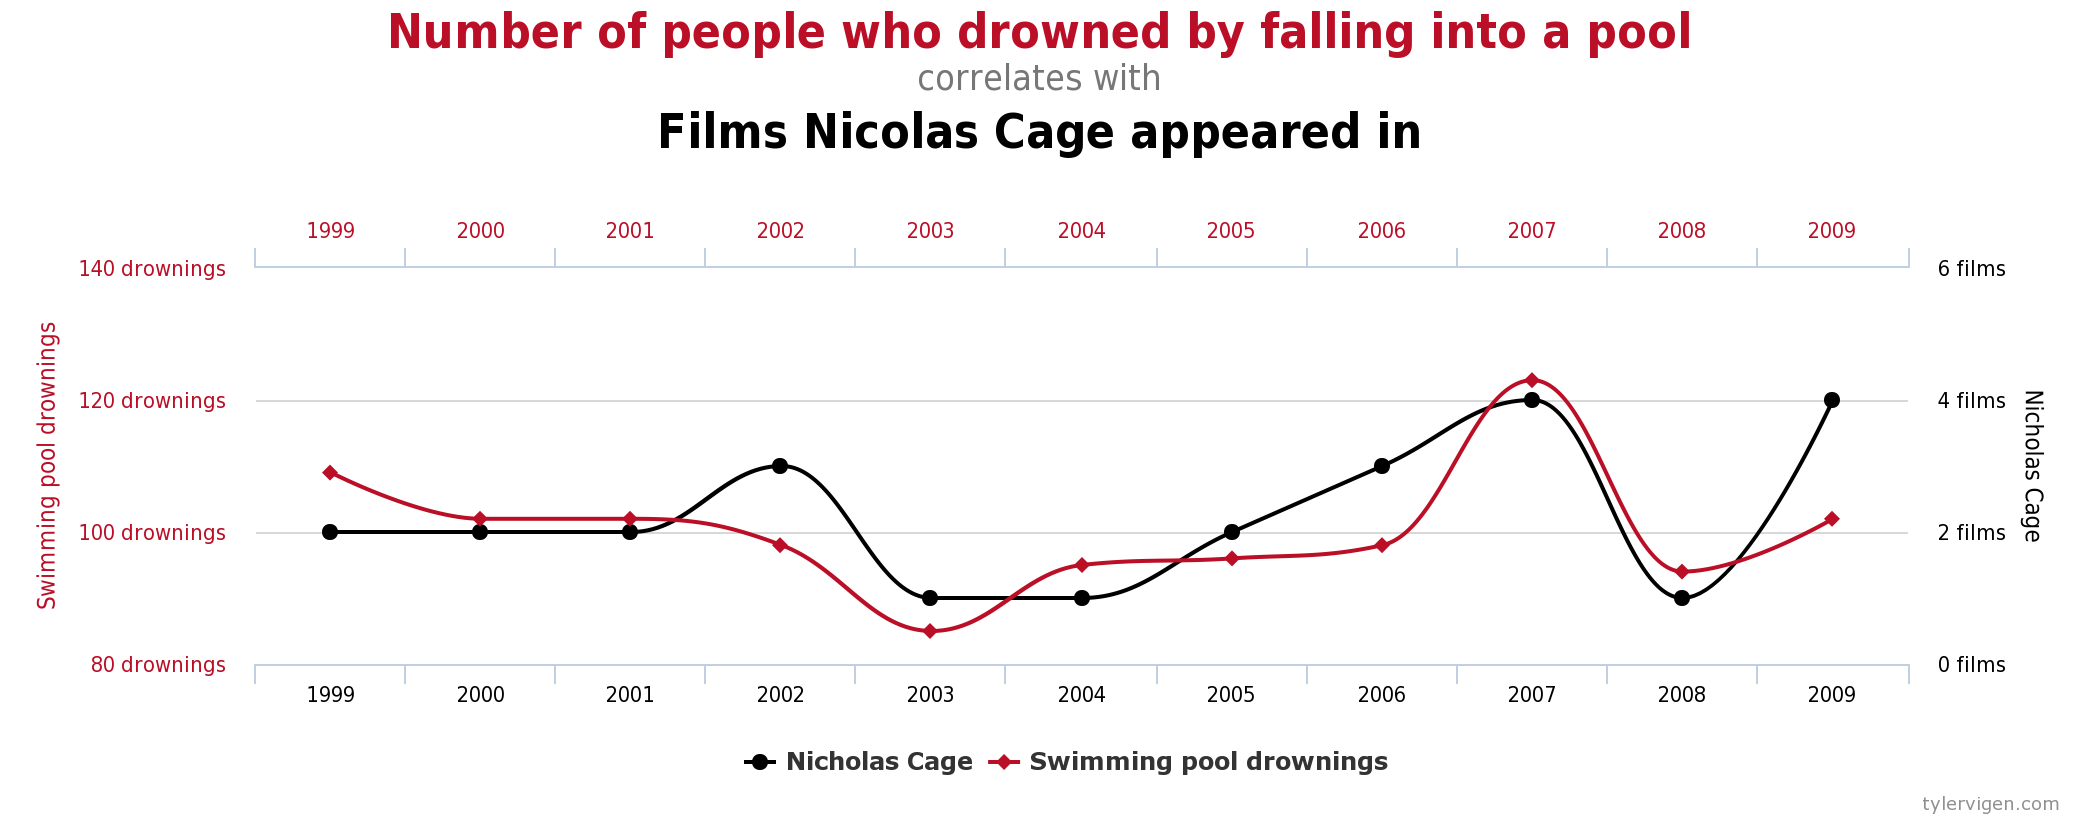
\includegraphics[width=0.8\linewidth]{rys1.png}
\caption{Fałszywe korelacje}
\label{fig:korelacje}
\end{center}
\end{figure}
Od lewej strony przedstawiono kolejne kroki obliczeń. Różne położenia punktów na osi oznaczają, że gdy ten mały zaczął krążyć, to ten duży nie mógł zdążyć. Kolejna para ilustruje, że gdy ten duży nie mógł zdążyć, to ten mały przestał krążyć. W punkcie 3 widać, że duży mógł już zdążyć, więc mały znowu zaczął krążyć.

Podsumowując, symulacje ujawniają występowanie efektu sprzężenia zwrotnego. Wzór (\ref{eq:wzor_wazny}) okazał się bardzo ważny.

\begin{table}[]
    \begin{tabular}{|l|l|l|l|l|}
    \hline
    Nagłówek 1  & Nagłówek 2  & Nagłówek 3   &  \\ \hline
    bla bla bla & bla & bla &  \\ \hline
    bla bla bla & bla & bla &  \\ \hline
    bla bla bla & bla & bla &  \\ \hline
    bla bla bla & bla & bla &  \\ \hline
    bla bla bla & bla & bla &  \\ \hline
    bla bla bla & bla & bla &  \\ \hline
    \end{tabular}
    \caption{Tytuł tabeli}
\end{table}


\section{Wnioski}
Odkryty efekt sprzężenia zwrotnego wskazuje wyraźnie na fakt, że co trzeci Polak jest przekonany, że jest co drugim Polakiem. Dodatkowym potwierdzeniem jest wysoka wartość stałej Laplace'a. Rozwiązano zatem problem postawiony w punkcie \ref{sec:wstep}.


\appendix
\section{Dodatek}
Kody źródłowe umieszczone zostały w repozytorium github:

\noindent \url{https://github.com/jdrapala/sieci_zlozone}.


\end{document}
